% Drawing 154/08-22 -- folder 154, batch 08, archive page 152 (PDF page 153).
% Transcription: le troisième dessin, au crayon : un fuseau entre les deux pseudo-droites $D$ et $D'$, coupé de droites, et un chemin brun en zigzag qui va d'une rive à l'autre de croisement en croisement
% Kind: spindle between D and D' with a zigzag path. Method 2 (schematic redraw from the facsimile). Status: partial.
% Notes: The spindle from its left tip (a marked point) to its right tip, the upper bank D with five marked vertices and the lower bank D' with four; the brown zigzag from the first upper vertex down to the first lower one and so on, with an arrowhead at each upper vertex, and a last brown arrow from the fourth lower vertex up to the fifth upper one; the letters D and D' at the right. The pencil lines of the arrangement through the vertices are left out; the lower edge of the spindle is cut by the bottom of the crop. Redrawn 2026-11-12 (issue 128): to check again. 2026-11-14, Claude Opus 5.5, overlay check (issue 147): rasterised from its own coordinates over the 400 dpi colour scan (402 ppi native) on a unit grid; not compiled (no TeX in the session). The spindle, its eleven marked points, the brown zigzag with its arrowheads and the letters D, D' lie on their ink to within about 0.5 unit; the redraw is unchanged. Still partial: the pencil lines of the arrangement (the « droites » that cut the spindle in the transcription: a small cross of two strokes above each upper vertex, long faint lines at the left, in the middle and at the right) and a faint pencil line inside the spindle from its left tip are not drawn.
% Coordinates: 1 unit = 1 mm = 1/100 of the crop width (bbox in page fractions: [0.12, 0.5, 0.6, 0.6]).
% Redrawn by Claude (claude-fable-5-2), issue #128, 2026-11-12; not checked by a human; not compiled (no TeX in the session).
% Checked by Claude (claude-opus-5-5) 2026-11-14 (issue #147): overlaid on the 400 dpi colour facsimile; not compiled (no TeX in the session). Not checked by a human. Status: partial.
% Rights: reproduces part of the work -- behind RENDER_TRANSCRIPTS, never published by itself.
\documentclass[tikz,border=3pt]{standalone}
\usepackage{amsmath,amssymb}
\usetikzlibrary{patterns,arrows.meta}
\tikzset{Br/.style={brown!80!black}, pencil/.style={black!45}, struck/.style={black!35}, mpt/.style={circle,draw,inner sep=1.3pt}, pt/.style={circle,fill,inner sep=0.9pt}, opt/.style={circle,draw,fill=white,inner sep=1.1pt}}
\begin{document}
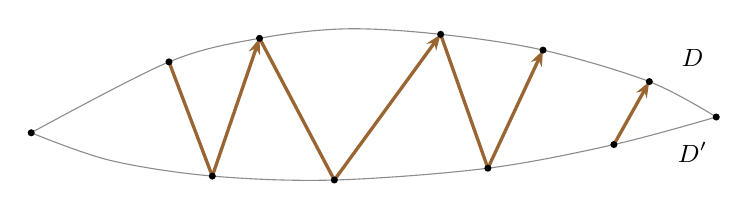
\begin{tikzpicture}[x=1mm,y=1mm,line cap=round,line join=round,font=\scriptsize]
\draw[pencil] plot[smooth, tension=0.55] coordinates {(12,-23) (29.5,-14) (41,-11) (52,-9.8) (64,-10.5) (77,-12.5) (90.5,-16.5) (99,-21)};
\draw[pencil] plot[smooth, tension=0.55] coordinates {(12,-23) (22,-26.5) (35,-28.5) (50.5,-29) (70,-27.5) (86,-24.5) (99,-21)};
\draw[Br,very thick] (29.5,-14) -- (35,-28.5);
\draw[Br,very thick,-{Stealth[length=2mm]}] (35,-28.5) -- (41,-11);
\draw[Br,very thick] (41,-11) -- (50.5,-29);
\draw[Br,very thick,-{Stealth[length=2mm]}] (50.5,-29) -- (64,-10.5);
\draw[Br,very thick] (64,-10.5) -- (70,-27.5);
\draw[Br,very thick,-{Stealth[length=2mm]}] (70,-27.5) -- (77,-12.5);
\draw[Br,very thick,-{Stealth[length=2mm]}] (86,-24.5) -- (90.5,-16.5);
\node[pt] at (12,-23) {};
\node[pt] at (99,-21) {};
\node[pt] at (29.5,-14) {};
\node[pt] at (41,-11) {};
\node[pt] at (64,-10.5) {};
\node[pt] at (77,-12.5) {};
\node[pt] at (90.5,-16.5) {};
\node[pt] at (35,-28.5) {};
\node[pt] at (50.5,-29) {};
\node[pt] at (70,-27.5) {};
\node[pt] at (86,-24.5) {};
\node[inner sep=1pt] at (96,-13.5) {\small $D$};
\node[inner sep=1pt] at (96,-25.5) {\small $D'$};
\end{tikzpicture}
\end{document}
